\chapter{Implementation}
An overview will consider the implementation of the project as a whole. Details of challenges and core parts of the system are then presented. The chapter will end with a summary of the requirements, and how they were met.

\section{Overview}
After finishing the design specification, work began on implementing the software. A project plan was drawn up, outlining a four stage approach to implementation:

\begin{enumerate}
	\item \textbf{Stage 1} Two weeks for a working prototype of the client side.
	\item \textbf{Stage 1} Three more weeks to build a fully working application of phase 1 (requirement specification).
	\item \textbf{Stage 1} Two weeks to implement phase 2, the usability requirements.
	\item \textbf{Stage 1} One week to make crowd games possible, phase 3 of the requirements.
\end{enumerate}

The first three stages became mixed, as their separation proved more of a hassle than benefit for reasons described below. Features were also advanced or postponed as their importance was re-considered. Below is a brief history of each of these stages.

Stage 1 was planned to be largely client side development. That meant adding the Angular framework to the HTML mock-ups created during the design. Its outcome would be a user interface complex enough to play a game, but only sitting on top of a dummy server API. After beginning development, it was soon apparent that some data needed to be persisted and updated by the server to properly create client software that communicated with it. Going out of the way to produce a solution on the client that would have to be replaced when the server logic was created was not worth the effort.

So stage 1 and stage 2 merged. Instead of focusing on a client/server split, development followed a core-feature-first approach. For example, players need to be able to see and use cards, so the user interface was created displaying cards with buttons to use them. Then the server was enhanced to allow users to use ingredient cards only, as these were needed to create rations. Discarding cards was deemed less important, and implemented later.

Stage 1 and 2 finished a week early, which allowed time for usability testing to begin. This generated feedback leading to more features and fixes. However, the next stage, stage 3, was concerned with implementing the usability requirements, making the game easier to learn and play. These new features and fixes therefore fitted in well, leading to significant improvement of the user interface.

As usability testing grew, larger groups needed to test the game. That meant each player having their own machine to play on became less practical, and so stage 4, concerned with crowd games was needed about the time it was planned. Stage 4 took less than a week to develop, yet required extensive testing. That, however, is the subject of the next chapter.

In the rest of this chapter particular parts of the implementation of the project that were challenging or interesting will be picked out and discussed.

\section{Working with AngularJS}
Development began with the client side. While Ruby on rails development was familiar as a framework, a disadvantage of using AngularJS was that it was a new technology. It presented a learning curve that had to be overcome. On the other hand, an advantage was the readily available plug-ins. Once understood, these cut down on development time. Early on in the project considerable time was taken finding good plug-ins, and then assessing their usability before proceeding too far with any of them.

\subsection{Bootstrap Library}
Bootstrap is a third party library famous for providing a quick and neat solution to common user interface demands. It provides templates for buttons, pop-ups, drop-downs, icons and text formatting. Traditionally, however, some of the more complex features of Bootstrap were powered by jQuery \cite{jQuery}, a popular Javascript library to allow easy DOM manipulation. However, Angualar has a different approach to jQuery. Insead of using jQuery-like DOM manipulation to change the view, the view references model data. Angular therefore does not blend well with jQuery. JQuery DOM manipulation in Angular controllers is overwritten when as the view will be quickly updated, and therefore should not be used \cite{AngularOverBB}. Instead, Angular plug-ins create their own solutions. Fortunately such a plug-in was provided which powered the usual Bootstrap features using Angular solutions, see \cite{AngularBootstrap} for details.

One such Bootstrap feature is the Bootstrap popover. Unfortunately HTML could not be inserted into the Angular-Boostrap solution. No way around this was suggested in the documentation for the plugin. Further more no solution seemed to be available, other developers must have accepted this inability or created their own solutions. 

Angular allows developers to create custom directives. In the Angular world, a directive is a view helper module which performs actions on the DOM. The popover feature was not complicated, and so the solution reached for this project was to create a custom popover feature that inserted an HTML template. By using a directive a combination of Angular and jQuery could be used to generate a working popover, called a 'popup'. The directive is detailed in Appendix E.

\subsection{Alerts}
Alerts are an important usability feature of the application, giving feedback about actions the users perform. If a button click is not allowed, an alert will be generated to inform the user why nothing happened. To create the alerts, the application began by using Bootstrap alert templates. This is a small coloured box with text that is dismissable. 

This worked for a while, but alerts are generated quite often, and it became apparent that they should wait for a set amount of time before fading away. This was fairly easy to implement. When created, each alert was given a lifetime in seconds. The Angular Bootstrap library provided alerts that could be dismissed in this way. However, like the popovers, these alerts could not hold HTML content, and so could not be styled.

The solution was to create a service. In Angular a service is a module of code that performs an operation, such as HTTP requests, sending emails, or in this case, creating and removing alerts. Within a service jQuery can be used to access and manipulate DOM objects. This solution used standard Bootstrap alerts, but also managed how long they remained. Another feature that could be added were batches of alerts. Some complicated server actions responded with a list of messages to display. The custom service checked if it was receiving a list, or a single message object and displayed them accordingly. The service is detailed in Appendix E.

\subsection{Restangular}
There are several Angular plug-ins that perform HTTP requests and handle the responses. The most basic is the \$http service, built into Angular itself. There are others, however, that are designed to work with RESTful API's, and provide short cuts for CRUD operations. Two of these were used, the Resource \cite{AngularResource} plug-in and Restangular \cite{Restangular}.

The first, Resource, seemed adequate. It enabled creating a service for each type of resource provided by the API. To query the resource, update or delete it, the service could be used, acting as a proxy to all requests to the server. For example, to request \textit{users/1}, a User service could be created with configuration set to access the \textit{users} route. It would map the get, update or delete functions to the correct resource route. This plug-in had one major shortcoming: it did not manage nested resources efficiently. To request users belonging to a game (\textit{games/1/users/1} with a RESTful API), a new GameUser service had to be created. Nested resources were key in the design of the server API, so another plug-in would be needed, if available, that could handle them.

The second plug-in, Restangular, did provide this support. Instead of treating every resource on the server as a service on the client side, it took a different approach. It provides a service from which any resource can be requested by using either a \textit{getList} method to request a collection, or a \textit{one} method with an id to request a single resource. These can be chained together to request nested resources. When a resource is returned, it is given the same attributes as the service. So while having the data of the resource provided by the API, it can also make the standard HTTP calls, thereby updating or deleting itself. This allowed a resource to be loaded and displayed to the user with little ground work.

It also meant that the client became much more dependent on the server and API. Very little data manipulation was needed by the client. When the model changed, a resource loaded could simply be updated by a patch request to the server, and then performing a get request to re-load it. This lead to the merger of stage 1 and 2 during development, already mentioned above.
	
\subsection{Storage and Security}
Another plug-in was used for client side storage. Storage is used to provide a session for the user. This is because the server API should be stateless, yet to protect user's security, authorisation is needed to access and update almost all resources. The best way to accomplish this is to require a user id and key in the header of all HTTP requests \cite{APISecurity}. Without these details requests will be returned with a 401, unauthorised, status.

So how does the user provide these details in the header? A login action, within the users controller, is outside the authentication check. This action checks the given user name and password, and if they match, returns the user details with an access token included. That access token is then used to validate user requests until they next login. Using an access token is a secure way of requesting a secret key that does not require the user to send their password with each request.

All actions on the server, but for login and registration, therefore have an associated user. That user can be checked against the information being requested, or updated, to verify that they have permission to access or amend the data. If a request is updating a user, game user, game user card's or a food ration, the ownership of the object can be checked. If users are updating game details, the system can check if they are the owner, if the request is ending the current turn, the system can check if it is in fact the authenticated user's turn. All this can be done without a session, simply with a user ID and secret token. Implementing this type of security is known method outlined for RESTful applications \cite{APISecurity}. The solution used is detailed in Appendix E.

Coming back to storage, it is therefore used to hold user details, including the access token, on the client side. This means that a session is maintained in the client without the server needing to know about it. There are two types of client side storage, session storage and local storage \cite{ClientStorage}. Both allow an application to store data in the web browser between page requests, making sessions easier and smoother to manage. Local storage is a persistent version of session storage, available to any tab and accessible forever, unless deleted by the application. There is a 5MB limit on storage per application. This is imposed by the browser.

Using the ngStorage plug-in \cite{reference}, either types of storage can be accessed simply by writing values to a provided storage object. An application prefix can be added, so that all data stored is a child of the application place holder. This mitigates the risk of other applications using the same storage key and wiping out the user's session. Session storage was used for this project, so that if users restart their browser, they do not continue to be logged in. It was a useful plug-in that worked as expected and saved a lot of hassle converting values to and from string types as they are stored and retrieved.

\section{Positions, and their Complexity}
As explained in the previous chapter, the game board is represented on the screen as a single image. In order to move food rations around, locations are identified by coordinates stored in the database as positions. A food ration therefore has a single location, allowing it to be positioned on the screen. 

When a player wants to move a food ration from one position to another, available positions must be highlighted, from which the user can choose one. Within the database, positions have the structure of a graph, with nodes and links between. To search for all the available positions the graph must be traversed up to a prescribed depth, and the response returned to the client.

\subsection{A Recursive Search}
The first attempt at traversing this graph took a recursive approach. A tree was constructed, using the starting node as the root, each link was followed and added to the tree. The tree was then encoded as JSON, sent to the client, and all it's positions rendered on the screen.

\begin{figure}[h]
\centering
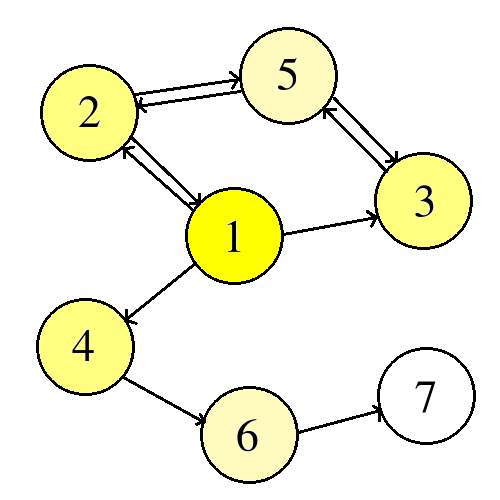
\includegraphics[width=2in]{Images/3/graph}
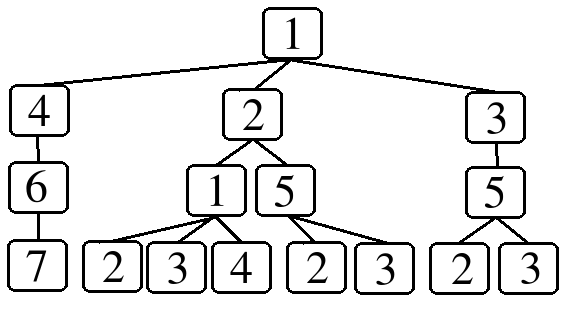
\includegraphics[width=2.5in]{Images/3/tree-1}
\caption{On the left is a visual representation of the arrangement of seven positions as a graph. On the right is a diagram of the result of a traversal on such a graph. Beginning at position 1, each link between nodes is followed until 3 steps (a depth of 3) have been taken. This tree would then be sent to the client, and each position drawn in place.}
\label{3_recursive_search}
\end{figure}

Unexpected and negative results quickly became apparent. The first and last positions were shown in a different colour, but did not appear where expected. This was due to the recursive traversal and display of the tree. Because some positions had two links between them, in opposite directions, the traversal could end up in a loop, or doubling back on itself. All the possible routes through the tree were being displayed, but this meant that when a neighbouring position was selected, the route to it may have gone through several other positions to get there.

\begin{figure}[h]
\centering
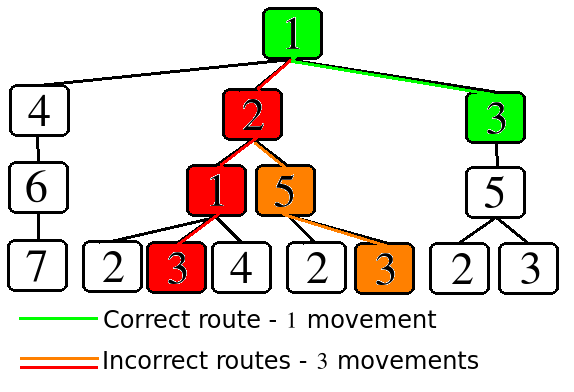
\includegraphics[width=3in]{Images/3/tree-1-example-1}
\caption{This shows how a tree was drawn by the client. No order was given for drawing, so starting with position 1, the right-most link was followed (order). Therefore positions to the right of the tree were hidden by the same positions drawn after. The position that should have been drawn first is shown in green, yet the incorrect routes, shown in red which take more movements, were shown.}
\label{3_recursive_search_wrong}
\end{figure}

If the problem involves positions occurring too many times, the first solution seemed to be checking if a position had been previously rendered, and if so, excluding it from the search. This was done on the server, but had even less usable results. Instead of showing all positions in the tree, only the first positions in the tree traversed were shown, but instead of improving the positions displayed, it introduced 'garden paths', where a random and unhelpful series of positions was chosen, this in turn created dead-ends and unreachable positions.

\begin{figure}[h]
\centering
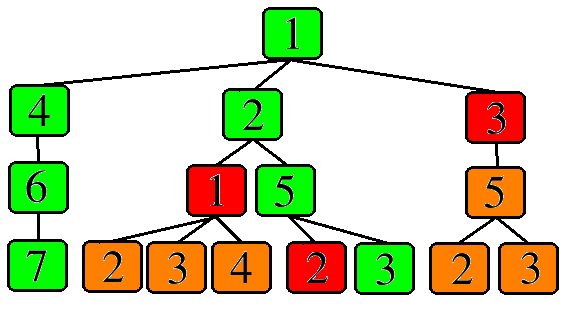
\includegraphics[width=3in]{Images/3/tree-1-example-2}
\caption{Positions in green are reached, positions in red are excluded because they have already been included. Positions in orange are not displayed because their parents are excluded. Once again, the shortest route to position 3 is not taken.}
\label{3_recursive_exclude_wrong}
\end{figure}

The problem lay with the recursive approach. To solve this, the graph had to be traversed in a different way.

\subsection{Traversing in Levels}
Instead of assembling the tree by following all possible paths until a certain depth, the tree must be built up in levels. The root node is added to a list of positions to display, and then all the positions it links to are added to the next level to check. When checking this level, if a position has not already been included, it is added to the list of positions to display and positions it links to are added to the next level to check. This continues until the specified depth is reached.

\begin{figure}[h]
\centering
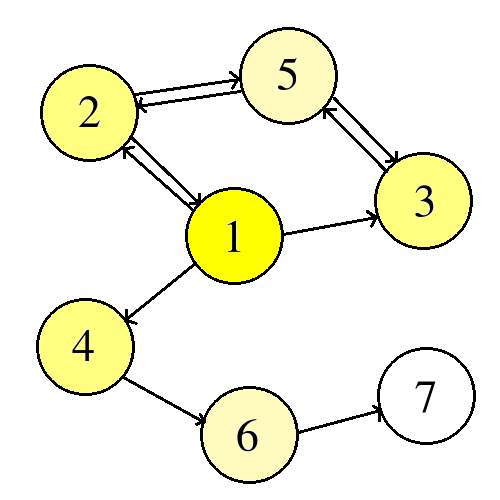
\includegraphics[width=2in]{Images/3/graph}
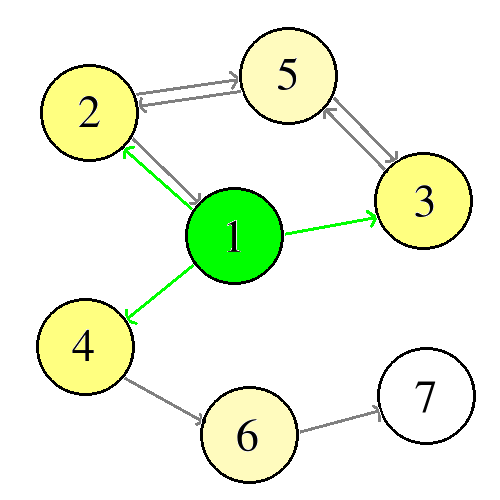
\includegraphics[width=2in]{Images/3/tree-2-step-1}
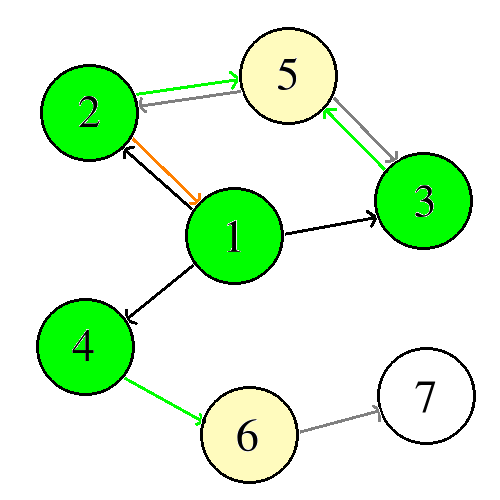
\includegraphics[width=2in]{Images/3/tree-2-step-2}
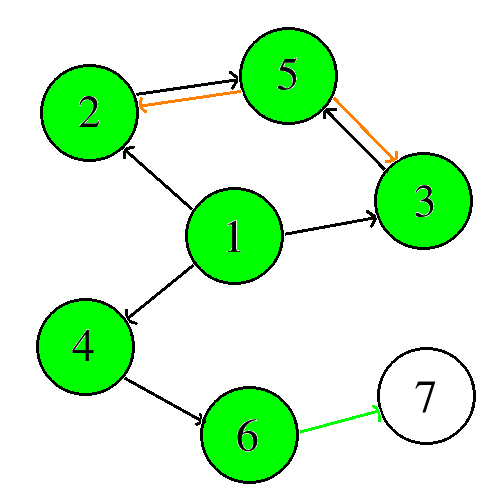
\includegraphics[width=2in]{Images/3/tree-2-step-3}
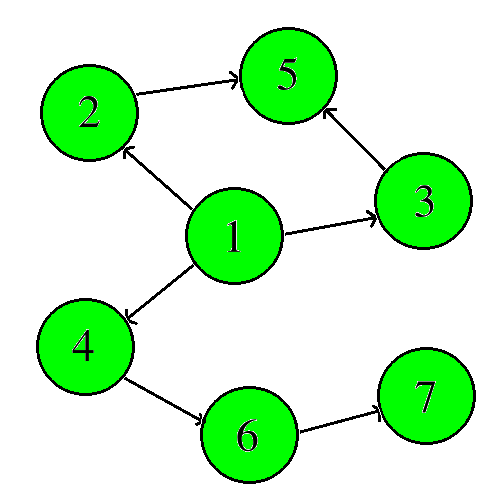
\includegraphics[width=2in]{Images/3/tree-2-step-4}
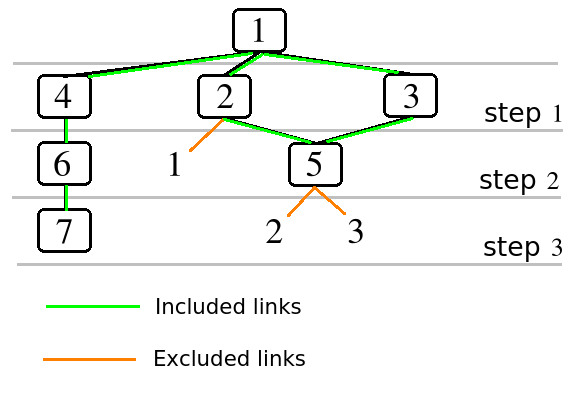
\includegraphics[width=2in]{Images/3/tree-2-full}
\caption{Steps of traversing the example graph, one set of links at a time. The resulting tree is shown at the end.}
\label{3_levels}
\end{figure}

This was implemented on the client. The server returned a recursively built tree, these were the allowed positions. The client built these into a graph, and then traversed the graph in the manner described above to render them. 

As a solution it worked, positions were displayed correctly, and it is still the method used by the system. However, there were several more improvements to make. Most notably, with a depth of ten or more, building a tree on the server and then constructing a graph on the client and traversing it took some time. It was too inefficient.

\subsection{Improving Efficiency}
The inefficiency was due to the traversal algorithm undergoing several changes. By this point the server was traversing the graph to find all the possible positions. These positions were being sent to the client where the graph was built and then traversed in the correct method described above. When a large depth was required, this could take some time to render. Latency in displaying the positions was due to the recursive method still being used on the server. Many positions appeared in the tree multiple times, the larger the depth, the more often they were included. Both the time it took for the server to build the tree, and send a gigantic package of JSON could add minutes to the process.

\begin{figure}[h]
\centering
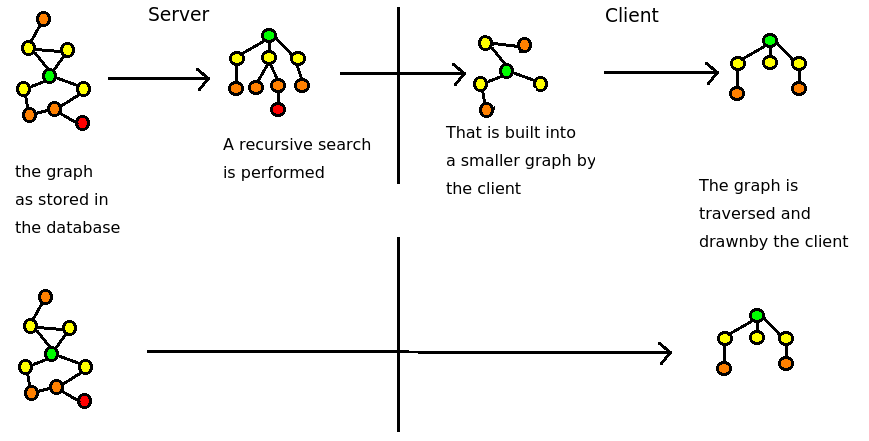
\includegraphics[width=5in]{Images/3/efficient-example}
\caption{The inefficient, previous method is shown above. The method below shows the change, which made rendering positions much faster. The most expensive step was building a recursive tree of possible positions. Consider a block of positions, each with four links. This can quickly create a maze of possible solutions. The recursively built tree tried to represent every route, whereas a tree built in layers merely presented an allowed subsection of the graph.}
\label{3_efficient}
\end{figure}

The solution was to remove an extra traversal and build step, shown in figure \ref{3_efficient}. Differences in speed were huge. The new solution experienced hardly any waiting time, compared to several seconds or minutes previously.

\subsection{Checking for Obstacles}
The task of rendering positions was complete. A further advantage, however, of moving the traversal to the server is worth considering. It was the ability to check the movement of food rations. A food ration can move a number of positions in a turn. To begin with, all movements were made by the client, and when finished the server was updated with the final position. Other elements in the digestive system become obstacles for food rations. 

Rather than relying on the client to recognise these objects, and prevent users clicking to move their ration on those positions, the checks could now be performed on the server. Clients are much more malleable and their restrictions are easily circumnavigated. While it is unlikely that someone would hack this application in order to cheat, best practice requires the server to validate user actions without relying on the client's suggestions \cite{APISecurity}.

A requirement, based on the original rules of the game, made avoiding obstacles more complicated. Food rations cannot normally move over each other, they provide obstacles for other rations. If, however, one ration has more fibre ingredients than another it may push past another ration. With checks implemented on the server, obstacles in the shape of food rations could be compared to the food ration on the root position. If they have less fibre ingredients, then they are no longer considered obstacles.

Delving to this depth into the display of positions was an aspect of the project that had not been considered during the design phase. It proved a challenging, yet rewarding, puzzle in which the benefits of different ways of traversing a graph were explored. The final algorithm for traversing the graph of positions is detailed in Appendix E.

\section{Card and Event Actions}
Cards specifying actions for the players to carry out are often used in board games. When such a card is played, it is usually trivial to carry that action out. To build the same rules into an application, however, is a different matter. Especially if the cards require further user input.

\subsection{Complex Specific Actions}
Both cards that players hold in their hand, and events which happen at the start of each round include actions. Some examples from the board game are:
\begin{itemize}
	\item \textit{'Move the pH marker up or down 1 to 3 squares, your choice.'} That seems simple, but how does the application query the user's choice? A form is needed where the user can specify whether they want the marker to move up or down, and one, two or three places. With the form comes the need for a special server action to process the results.
	\item \textit{'Change up to two ingredients of any player's food ration by the same number from your hand.'} This is more complex still. It requires first a form where a user picks a food ration, and then one or two ingredients. The player must then be presented with a choice of ingredients to discard, up to the same number.
	\item \textit{'All rations that leave the rumen this turn have up to one fibre ingredient turned into protein.'}  This does not require user input, but it does need a way of recording that the card has been played in a round, and to check each ration that moves past a certain position. That means an extra value, or record in the database just for a card action.
\end{itemize}
	
Some actions were easier, involving moving a few values of a cow record up or down, or changing a player's score. These were implemented by performing an action based on the type of card when the request comes to the server for it to be used. The rest of the actions had to be simplified, so that they did not require user input, and could be completed in the scope of the project.

\subsection{Cow Events}
As well as one off actions, some events cause an ongoing effect. These are categorised as weather, disease or pregnancy events. In each of these cases the event remains active until it is replaced by another event. For example, a weather event such as 'Hot Weather' remains active. This is achieved by setting a value in the cow record called 'weather\_event' to the id of the event. That is strait forward, the difficult part is making sure its action is carried out. It must be performed whenever relevant while the event remains.

To do this, each persistent event was given a helper method in the cow model. The method returns a boolean value, indicating whether the event is active. Throughout the code base, these methods can give an indication of the state of the cow, while keeping in one place the logic to check if the event is active. An example is constipation or diarrhea in the intestines of the cow. When deciding how far a food ration can move, a test is needed to see if either of these diseases are active. If so a further check is carried out to test whether the ration is in the intestines. If so, its movement is affected.

Having considered server functionality, the client interface also took a large section of implementation time. Aspects of it are well worth discussing.

\section{Updating The Client}
Beyond the plug-ins and learning curve provided by the client side framework, a feature of note not covered by the design, yet needing implementation was updating the client.

Synchronising the client and server was not covered in the design. As the server is stateless, all the initiative comes from the client. It is the client that requests data. The server merely processes a request and returns a result. Most of the time this is all that is needed.

However, when several people are performing actions on the same data within an application, updating every client with the latest data goes outside of the normal work-flow described above. This regularly happens within the application. As players take their turn, the data will change, and when they finish their turn, the server is updated and registers that it is the next player's turn. However, the next player's client will not be updated automatically. They will not know it is their turn without refreshing the page.

The issue lies with server-to-client communication. There are three potential solutions. It was a matter picking the simplest one that met the needs of the project.
\begin{itemize}
	\item One solution is for the server to somehow push an update whenever the state of certain objects change. This is possible between servers, but breaks the standards of client-server requests and is therefore unsupported. When searching for a way to implement this within the Rails framework, no documentation for an approach could be found within the Rails community. This suggested it is not a common approach.

	\item The second solution is for the client to perform a request, which the server holds until a change is triggered in an object. When that happens it returns the request with the updated data. The client can then update and perform another request. There is little support for this in Rails or Angular however.

	\item The third solution, which was implemented, was a regular update loop. When a game started, the client is set to perform a request every five seconds. This is a long enough wait to avoid over loading the server, yet is a natural enough period to wait for a page to change, based on some event.
\end{itemize}

With this in place, players can play games across a network without refreshing the page once.

\section{Crowd Games}
Phase three of the requirements analysis covered crowd games. They are games where players take turns to perform actions at one client, instead of playing across a network using multiple clients. Challenges were perceived when it came to implementing this new dynamic, but in event it was not too arduous a task.

\subsection{Designing for Crowd Games}
As crowd games were always in the list of requirements, they were built into the design of the user interface. 

The biggest question was how to securely manage accounts when many players needed to be logged in at once. It was planned that when creating a crowd game, the set up page would require a user to log in before they could join. This prevents a user being added to a game without their permission.

When users login, their details are stored in an object in the base controller, from which all other controllers extend. Every time the authenticated user's details were used during implementation, they were sourced from this object. When a user logs out, the details of this object are erased. This design helped to keep the concerns of user authentication in one place.

\subsection{Changing Accounts}
When it came time to implement crowd games, properly authenticating and changing between users was simple. When the game is created users authenticate themselves. These details are kept in local storage as a list of users who are playing the game. When a player ends their turn, the id of the next player is returned by the server. The list of players is searched for that id, and the player is authenticated and their details fetched.
	
\subsection{Changing User Authentication}
Once crowd and single games were implemented, a cleaner design was conceived with two types of user account that could be authenticated. It became necessary to separate the account within a game, from the account of a player who had logged in to view their games. This was because, when playing a crowd game, a player could return to the main menu, and the authenticated player would be the player whose turn it currently is in the crowd game.

To avoid players being logged in through a crowd game, a user was defined as someone who authenticated themselves to view information, such as their list of games or profile. Whereas a player was the person currently authenticated and taking their turn in the game. In a networked game, when a user resumes a game, they become the player as well. The player account can be changed without affecting the user who is logged in. This helped simplify management of accounts in crowd games.

With this separation of accounts the possibility arose to remove the distinction between games altogether. When a game is begun players could choose to login on the same machine, or take a networked approach, the game could then either automatically log the player in, or wait for them to take their turn, if they have not authenticated themselves.

This unification of game types actually simplified the process of setting up games had a threefold advantage. First of all, instead of asking a player to choose between two types of games, and explaining the differences, game creators merely have to define players as being at the same machine as them, or distant across a network. Users can begin a game across a network, but resume it later, together at the same machine. 

The second benefit is that there was no real difference between networked and crowd games, but their set up. By combining the games the set up pages of crowd games could be removed. Any future changes did not have to be replicated across two types of set up page.

The final benefit was that by making the games operate in the same way many of the issues of distinguishing between crowd or networked games in the code were removed, making the code simpler. This was already done by the system, but it also had to work out what type of game was being played, and unnecessary burden. The flexibility of assigning users as distant or present more naturally fitted the design of the system.